
\documentclass{beamer}
\setbeamertemplate{navigation symbols}{}
    \addtobeamertemplate{frametitle}{\vspace*{-0.1cm}}{\vspace*{-0.5cm}}

\setbeamercolor{frametitle}{fg=black,bg=white}
\setbeamertemplate{caption}[numbered]
\usetheme{CambridgeUS}
\usepackage{ngerman}
\renewcommand{\figurename}{Figure}
\renewcommand{\tablename}{Tabel}
\newcommand\numberthis{\addtocounter{equation}{1}\tag{\theequation}}
\newcommand\norm[1]{\left\lVert#1\right\rVert}
\usepackage[utf8]{inputenc}
\usepackage[T1]{fontenc}
\usepackage[backend=biber]{biblatex}
\bibliography{literature_seminar.bib}

% Removes icon in bibliography
\setbeamertemplate{bibliography item}{}


\begin{document}
\title[Deep Taylor Decomposition]{Explaining NonLinear Classification Decisions with Deep Taylor Decomposition by Montavon et al.}  
\author{Marcel Pommer}
\institute[LMU M\"unchen]{Ludwig-Maximilians-Universität M\"unchen}
\date{\today} 

\begin{frame}
\titlepage
\end{frame} 

\begin{frame}
\frametitle[Explainability]{Explainability}
\vspace{0.25cm}
\begin{figure}
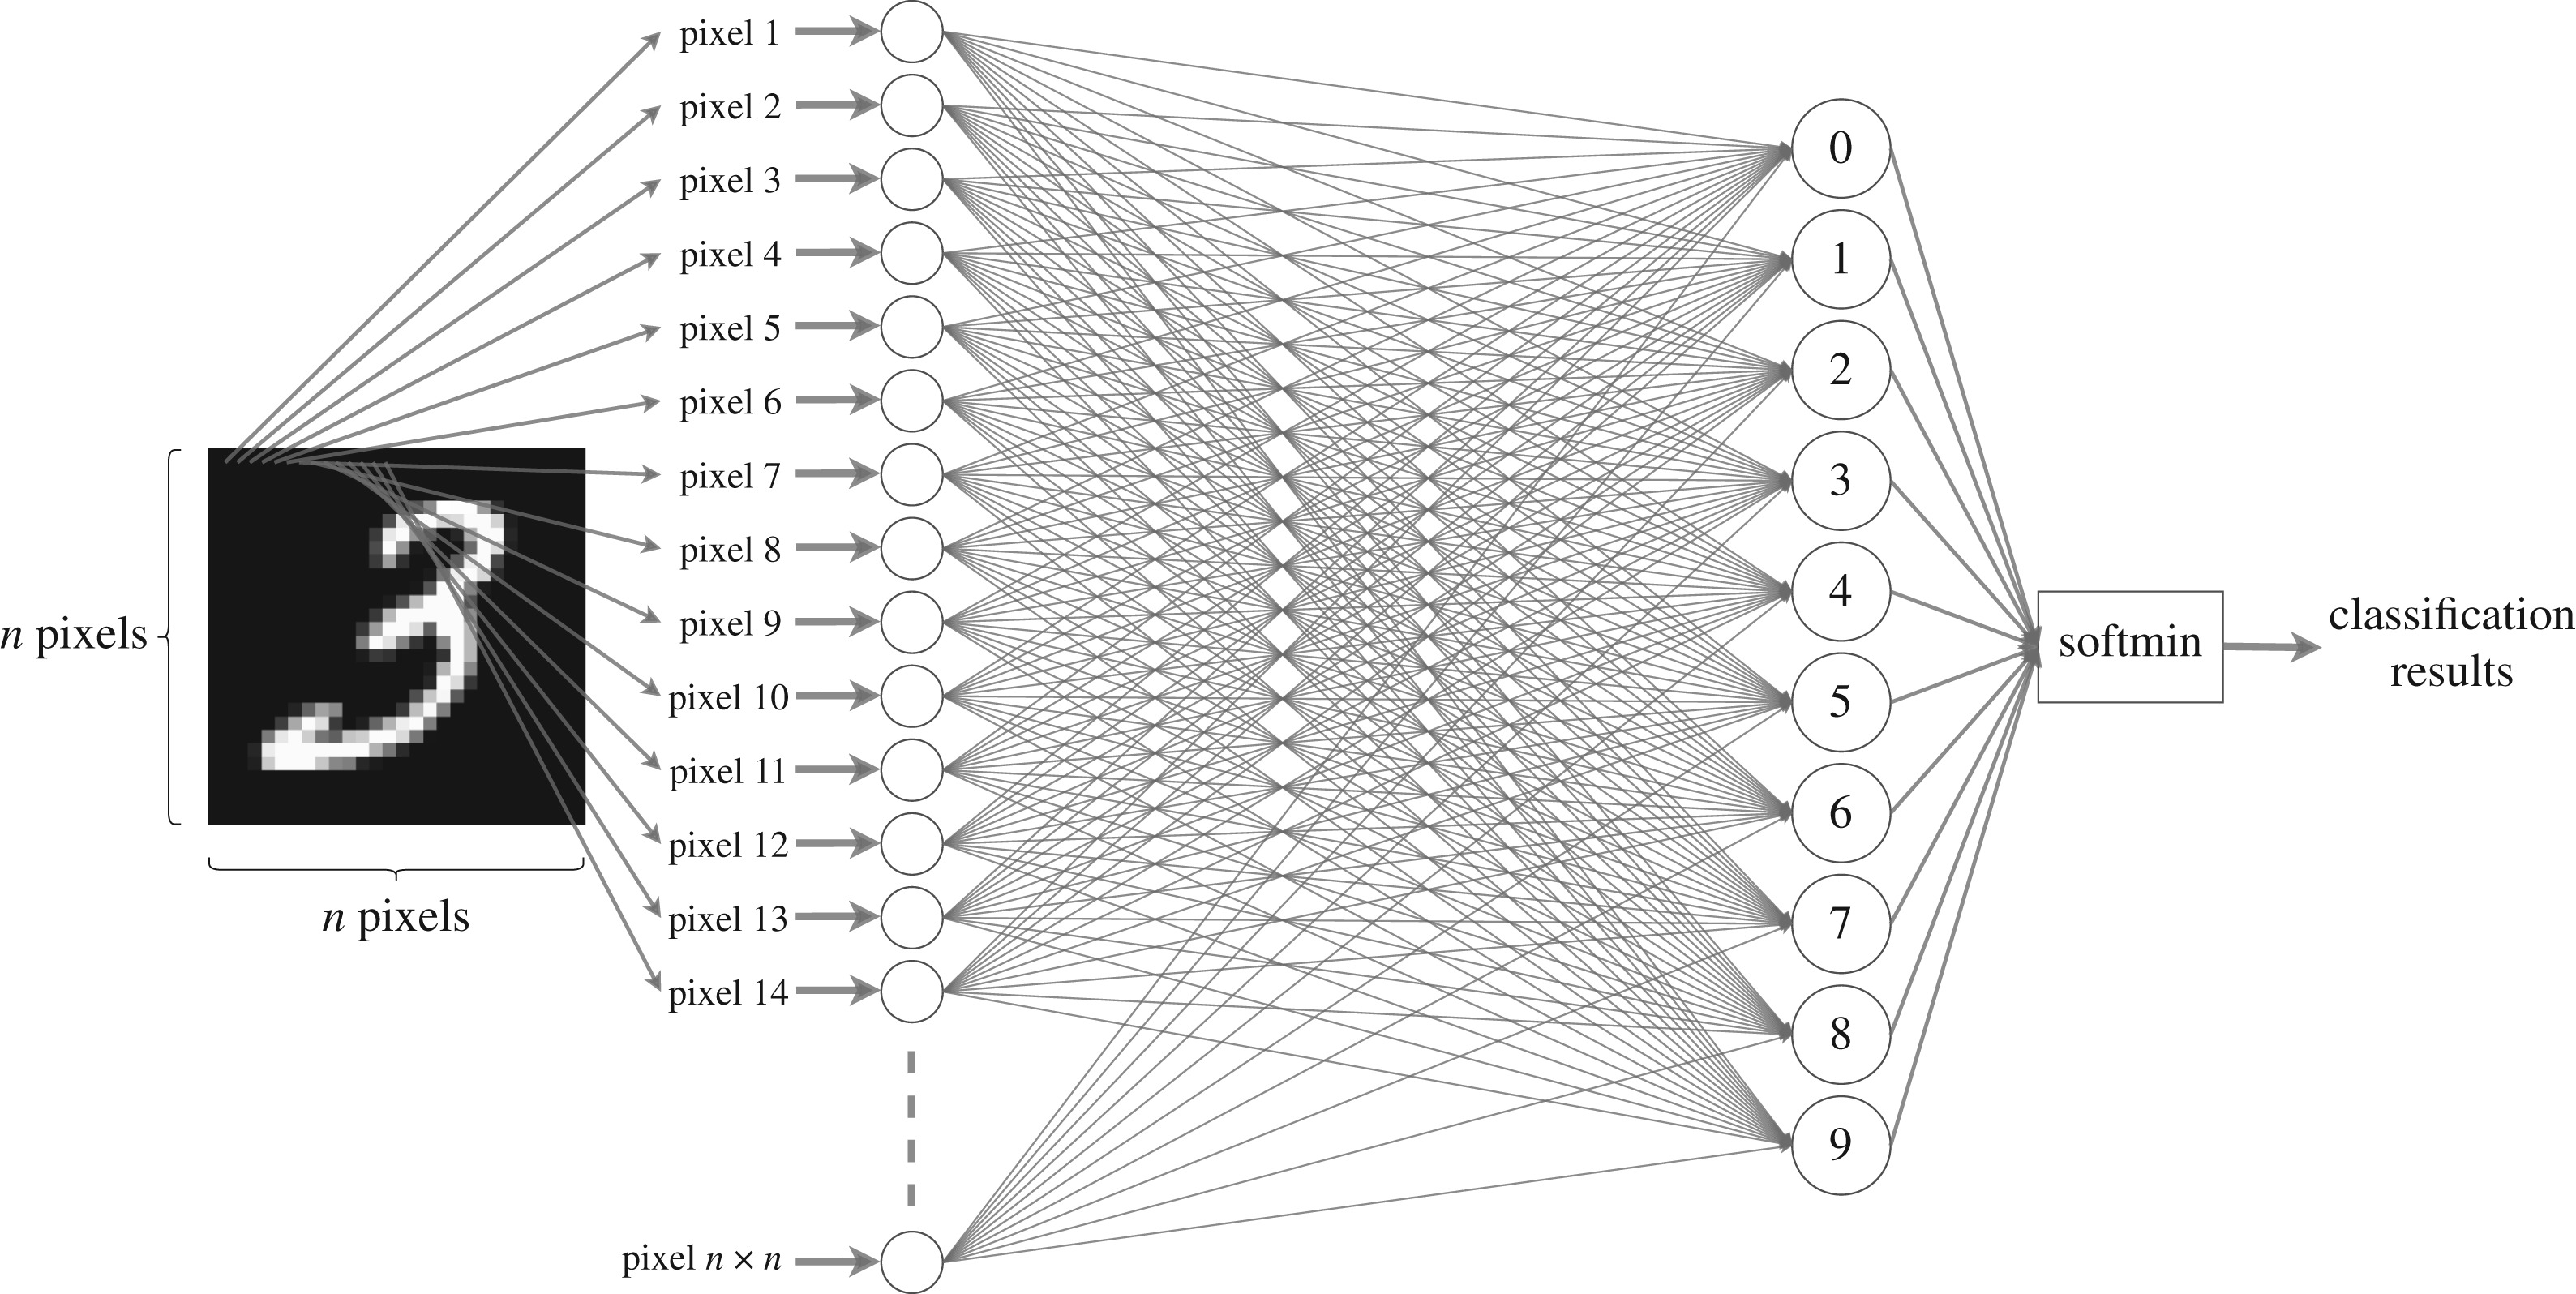
\includegraphics[width=0.9\textwidth]{image/introduction_image}
\end{figure}
\vspace{0.25cm}
Deep neural networks perform great on a variety of problems \nocite{*}\\
\textbf{but} how can we explain decisions made by complex deep architectures?\\
\end{frame} 


\begin{frame}
\frametitle[Table of Contents]{Table of Contents}
\vspace{0.4cm}
\tableofcontents
\end{frame} 

\AtBeginSection[]
{
\begin{frame}
\frametitle[Table of Contents]{Table of Contents}
\vspace{0.4cm}
\tableofcontents[currentsection]
\end{frame} 
}


\section[Introduction]{Introduction}
\begin{frame}
\frametitle{Introduction} 
\textbf{Deep neural networks revolutionized amongst others the field of}\\
\vspace{0.25cm}
       \begin{columns}[T]
          \column{0.62\textwidth}
             \centering
             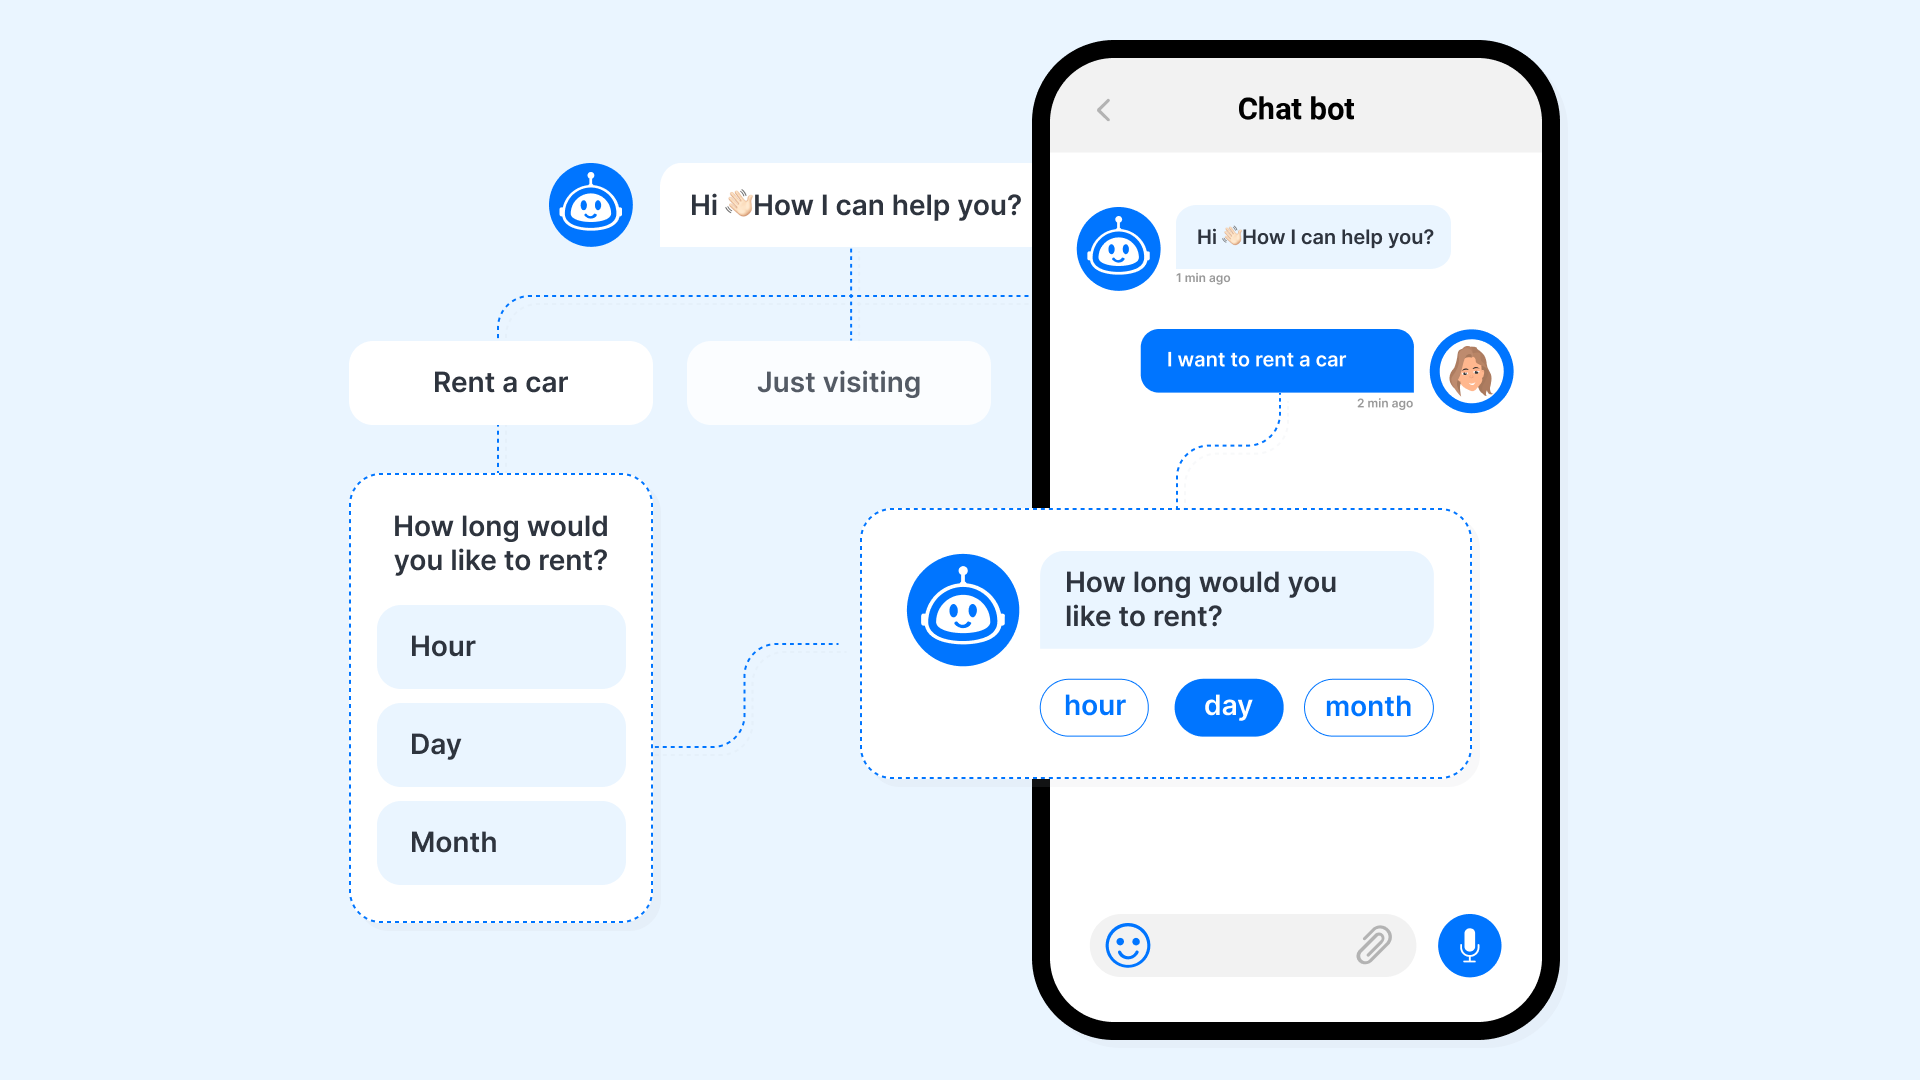
\includegraphics[height=5cm, width=8cm]{image/NLP_chatbot}
           \column{0.35\textwidth}
			\begin{itemize}
			\item[--] Image recognition
			\item[--] Natural language processing
			\item[--] Human action recognition
			\item[--] Physics
			\item[--] Finance
			\item[--] ...
			\end{itemize}
         \end{columns} 
\pause
\vspace{0.5cm}
With one major drawback $\rightarrow$ \textbf{lack of transparency}
\end{frame}


\iffalse

\begin{frame}
\frametitle{Interpretable Classifier} 
\vspace{0.5cm}
Explanation of non-linear classifiers\\
$\rightarrow$ A classifier should not only provide a result but also a reasoning

\begin{center}
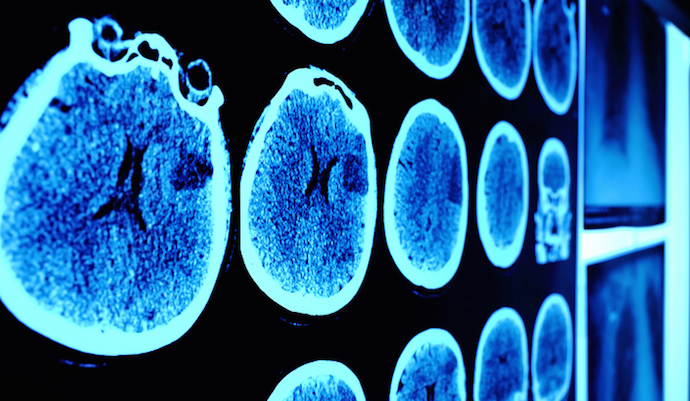
\includegraphics[height=5cm, width=8cm]{image/cancer}
\end{center}

We do not only need to know if the patient has cancer but also where exactly it is located

\end{frame}

\fi




\begin{frame}
\frametitle{General Idea} 
\vspace{0.5cm}
To accomplish the task of explainability we map relevance from the output to the input features

\vspace{0.25cm}

\begin{center}
\begin{figure}
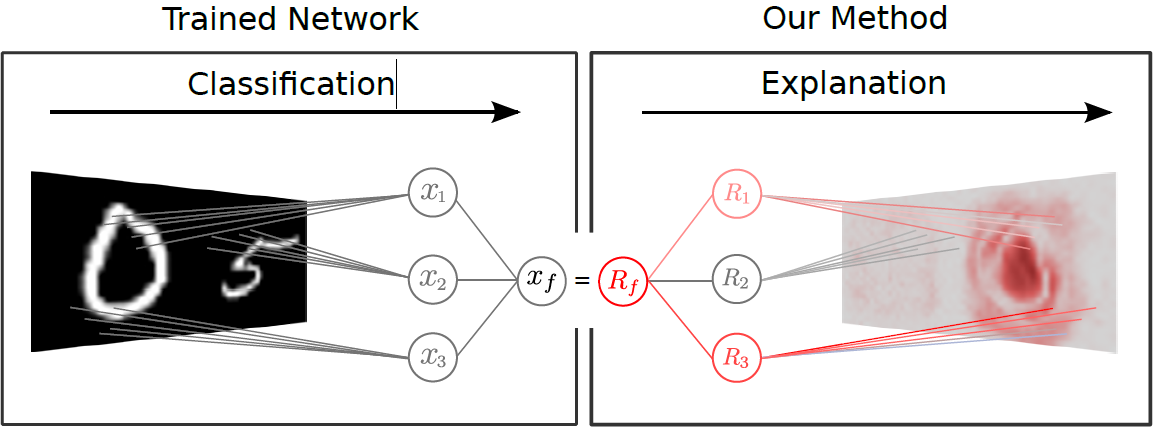
\includegraphics[height=4.5cm, width=11cm]{image/fig._1_example}
\caption{Neural Network Detecting 0 while Distracted by 5}
\end{figure}
\end{center}

\end{frame}




\section[Pixel-Wise Decomposition]{Pixel-Wise Decomposition}

\subsection[Mathematical Framework and Definitions]{Mathematical Framework and Definitions}



\begin{frame}
\frametitle{Mathematical Framework}

In the context of image classification we define the following mathematical framework
\begin{itemize}
\item Positive valued function $f:\mathbb{R}^d\to \mathbb{R}^+$, where the output $f(x)$ defines either the probability that the object is present or the quantity of the object in question
\item[$\rightarrow$] $f(x)>0$ expresses the presence of the object  

\pause
\end{itemize}

 \begin{columns}
          \begin{column}[T]{8cm}
          		\begin{itemize}
          		\item Input $x \in \mathbb{R}^d$, decomposable in a set of pixel values $x=\{x_p\}$
			\item Relevance score $R_p(x)$ indicating the relevance of each pixel
			\item[$\rightarrow$] The relevance score can be displayed in a heatmap denoted by $R(x) = \{R_p(x)\}$
			\end{itemize}

            \end{column} 
            \begin{column}[T]{3.5cm}
			\begin{figure}
			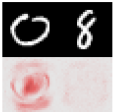
\includegraphics[height=2.75cm, width=2.75cm]{image/heatmap_example}
			\end{figure}
	\end{column}
\end{columns} 

\end{frame}



\begin{frame}
\frametitle{Definitions}
\begin{block}{Definition 1}
A heatmapping $R(x)$ is \underline{conservative} if the sum of assigned relevances in the pixel space corresponds to the total relevance detected by the model, that is
\begin{equation}
\forall x: f(x)=\sum_p R_p(x)
\end{equation}
\end{block}

\vspace{0.5cm}
\pause
\begin{block}{Definition 2}
A heatmapping $R(x)$ is  \underline{positive} if all values forming the heatmap are greater or equal to zero, that is:
\begin{equation}
\forall x,p: R_p(x) \geq 0
\end{equation}
\end{block}

\end{frame}


\begin{frame}
\frametitle{Definitions}
All algorithms are shall comply with definition 1 and 2\\
\vspace{0.1cm}


\begin{block}{Definition 3}
A heatmapping $R(x)$ is  \underline{consistent} if it is  \textit{conservative} and  \textit{positive}. That is, it is consistent if it complies with Definitions 1 and 2.
\end{block}


\vspace{0.5cm}

\pause
But consistency is not a measure of quality which can be seen on the following example which complies with definition 3
\begin{equation*}
\forall p: R_p(x) =\frac{1}{d} \cdot f(x) ,
\end{equation*}
where d denotes the number of pixels
\end{frame}



\subsection[Taylor Expansion and Sensitivity Analysis]{Taylor Expansion and Sensitivity Analysis}

\begin{frame}
\frametitle{Taylor Expansion}
\vspace{0.35cm}
First order Taylor expansion at root point $\tilde{x}$
\begin{flalign*}
 f(x) & =f(\tilde{x}) + \left( \frac{\partial f}{\partial x}\Big|_{x=\tilde{x}}\right)^T \cdot (x-\tilde{x}) + \epsilon\\
       & = 0 + \sum_p \underbrace{\frac{\partial f}{\partial x_p}\Big|_{x=\tilde{x}} \cdot (x_p-\tilde{x}_p)}_{R_p(x)} +\  \epsilon  
\end{flalign*}

\pause
The challenge of finding a root point
 \begin{columns}
          \begin{column}[T]{5.5cm}
             \begin{figure}
             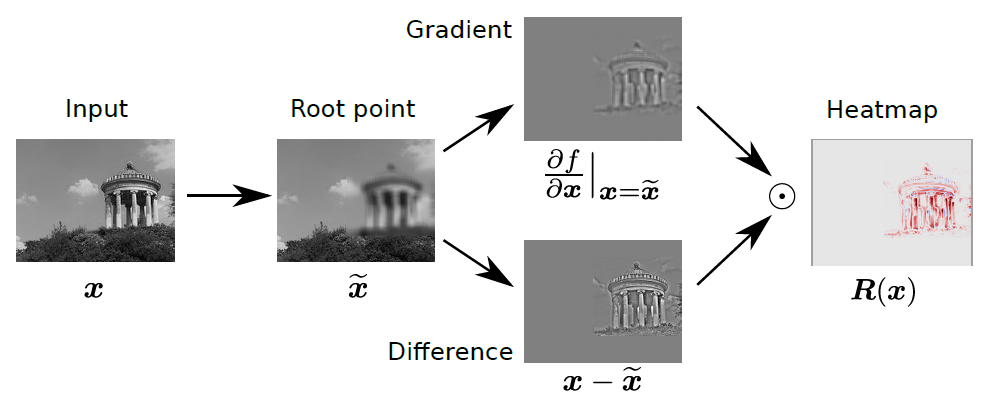
\includegraphics[height=2.75cm, width=6cm]{image/fig._2_example_root_point}
             \end{figure}
            \end{column} 
            \begin{column}[T]{6.2cm}
			\begin{itemize}
			\item Potentially more than one root point
			\item Remove object but deviate as few as possible
			\item[$\rightarrow$] $\min_{\xi} \norm{\xi-x}^2 \text{subject to } f(\xi)=0$
			\end{itemize}
	\end{column}
\end{columns} 


\end{frame}



\begin{frame}
\frametitle{Sensitivity Analysis}
\vspace{0.35cm}
Choose a point at infinitesimally small distance from the actual point, i.e. $\xi = x- \delta \frac{\partial f}{\partial x}$, where $\delta$ is small\\
\pause
\vspace{0.35cm}
If we assume a locally constant function we get
\begin{flalign*}
 f(x) & =f(\xi) + \left( \frac{\partial f}{\partial x}\Big|_{x=\xi}\right)^T \cdot (x- (x- \delta \frac{\partial f}{\partial x})) + 0\\
       & = f(\xi) + \delta \left( \frac{\partial f}{\partial x}\right)^T \cdot  \frac{\partial f}{\partial x} + 0\\
       & = f(\xi) + \sum_p \underbrace{ \delta \left( \frac{\partial f}{\partial x}\right)^2}_{R_p} +\ 0
\end{flalign*}

\pause
\begin{itemize}
\item The heatmap is positive but not conservative
\item The heatmap only measures a local effect
\end{itemize}



\end{frame}



\begin{frame}
\frametitle{Deep Taylor Decomposition}
\vspace{0.25cm}
\begin{figure}
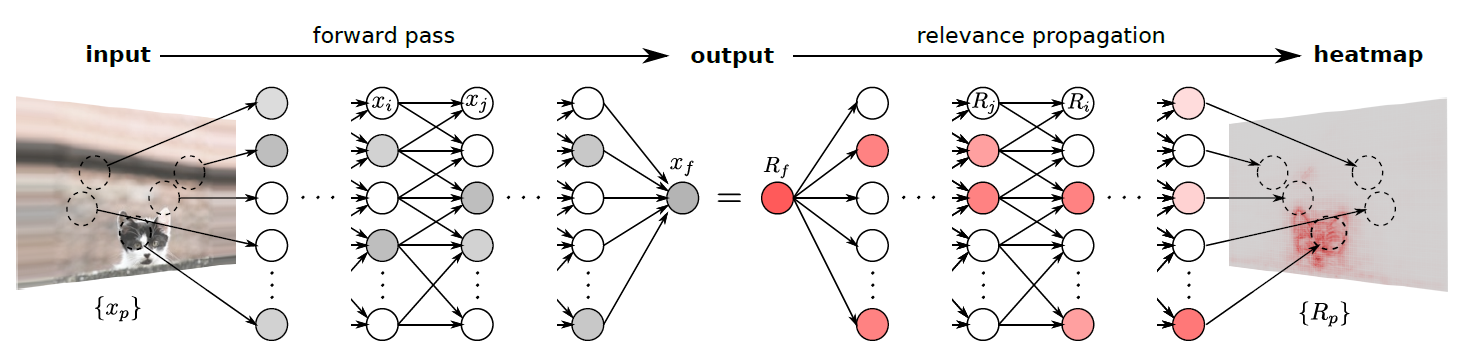
\includegraphics[height=2.75cm, width=11cm]{image/deep_taylor_decomposition_example}
 \end{figure}
\vspace{0.25cm}

\pause
We view each layer as a separate function and write the Taylor decomposition of $\sum_j R_j \text{ at } \{x_i\}$ as
\begin{align*}
    \sum_j R_j &= \left( \frac{\partial (\sum_j R_j)}{\partial \{x_i\}}\Big|_{\{\tilde{x}_i\}}\right)^T \cdot (\{x_i\}-\{\tilde{x}_i\}) + \epsilon\\
    &= \sum_i \underbrace{\sum_j \frac{\partial R_j}{\partial x_i}\Big|_{\tilde{x}_i} \cdot (x_i-\tilde{x}_i)}_{R_i} +\ \epsilon
\end{align*}
\vspace{-0.25cm}

\end{frame}

\begin{frame}
\frametitle{Deep Taylor Decomposition}
\vspace{0.25cm}
\begin{figure}
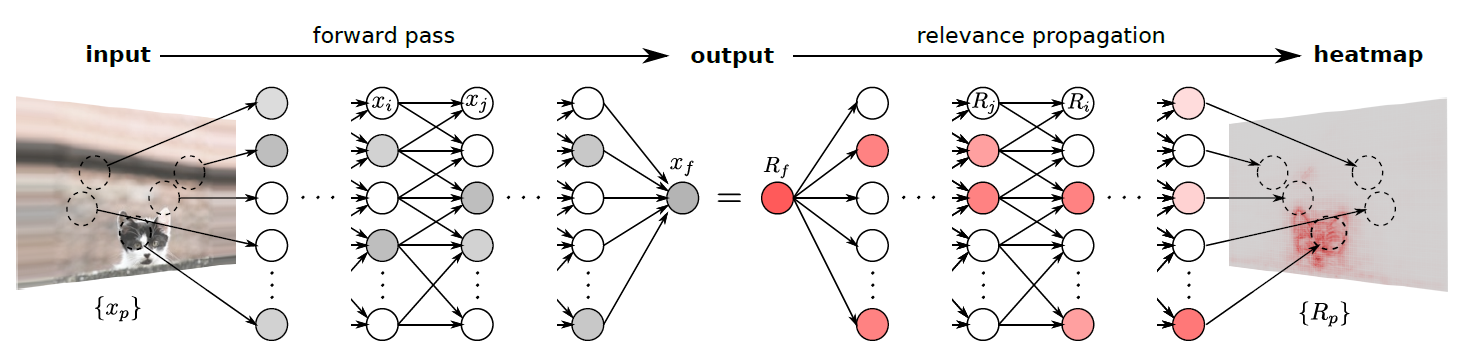
\includegraphics[height=2.75cm, width=11cm]{image/deep_taylor_decomposition_example}
 \end{figure}

\begin{itemize}
\item  If each local Taylor decomposition is \textit{conservative} then the chain of equalities is also \textit{conservative} (layer-wise relevance conservation)
\item[$\rightarrow$] $R_f = ...= \sum_i R_i = ... = \sum_p R_p$
\item  If each local Taylor decomposition is \textit{positive} then the chain of equalities is also \textit{positive} 
\item[$\rightarrow$] $R_f,...,\{R_i\},...,\{R_p\} \geq 0$
\item If each local Taylor decomposition is \textit{consistent} then the chain of equalities is also \textit{consistent} 
\end{itemize}


\end{frame}

\section[One-Layer Networks]{Application to One-Layer Networks and Root Finding}



\begin{frame}
\frametitle{Setting}
\vspace{0.5cm}

Consider a simple detection-pooling one layer neural network with
\vspace{-0.2cm}
 \begin{columns}
          \begin{column}[T]{5.5cm}
		\begin{align*}
		x_j &= \max(0, \sum_i x_i w_{ij} + b_j)\\
		x_k &= \sum_j x_j, \ b_j \leq 0, \forall j
		\end{align*}
            \end{column} 
            \begin{column}[T]{6.5cm}
			\begin{figure}
				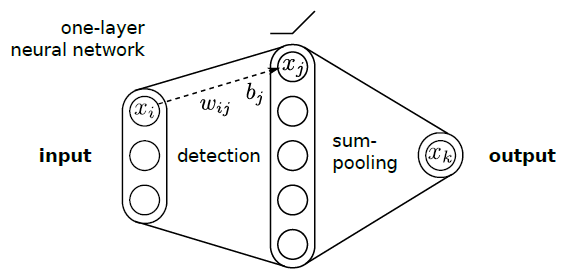
\includegraphics[height=2.5cm, width=6cm]{image/one_layer_nn}
			\end{figure}
	\end{column}
\end{columns} 
\vspace{0.25cm}

\pause
\begin{enumerate}
\item $R_k = x_k$ and thus $R_k = \sum_j x_j$
\item  Chose a root point and redistribute $R_k$ on neurons $x_j$\\
$\rightarrow$ $R_j = \frac{\partial R_k}{\partial x_j}\Big|_{\{\tilde{x}_j\}} \cdot (x_j - \tilde{x}_j) $, with $\{\tilde{x}_j\}=0$
\item Since $\frac{\partial R_k}{\partial x_j}\Big|_{\{\tilde{x}_j\}}=1$ we obtain $R_j = x_j$
\item Apply Taylor decomposition another time and get\\
 $R_i = \sum_j\frac{\partial R_j}{\partial x_i}\Big|_{\{\tilde{x}_i\}^{(j)}} \cdot (x_i - \tilde{x}_i^{(j)})$
\end{enumerate}



\end{frame}


\begin{frame}
\frametitle{Derivation of Propagation Rules}
\vspace{0.5cm}
Given $R_j = \max(0, \sum_i x_i w_{ij} + b_j)$ and $b_j \leq 0$ and a search direction $\{v_i\}^{(j)}$

\begin{equation}
\tilde{x}^{(j)}_i = x_i + t v_i ^{(j)} \Leftrightarrow t = \frac{\tilde{x}_i^{(j)} - x_i}{v_i^{(j)}}
\label{equ:search_direction}
\end{equation}

\pause
\vspace{0.1cm}
If $\sum_i x_i w_{ij} + b_j>0$ the nearest root along the search direction $\{v_i\}^{(j)}$ is given by the intersection of equation \eqref{equ:search_direction} and $\sum_i\tilde{x}_i^{(j)} w_{ij} + b_j=0$  
\begin{align*}
&               & 			0 &= \sum_i x_i w_{ij} + b_j + \sum_i v_i^{(j)} t w_{ij} \\[0.25em]
&\Leftrightarrow& -t & = \frac{\sum_i x_i w_{ij} + b_j}{\sum_i v_i^{(j)} w_{ij}}\\[0.5em]
&\Leftrightarrow& x_i - \tilde{x}_i^{(j)} & = \frac{\sum_i x_i w_{ij} + b_j}{\sum_i v_i^{(j)} w_{ij}} v_i^{(j)}
\end{align*}

\end{frame}




\begin{frame}
\frametitle{Derivation of Propagation Rules}
\vspace{0.4cm}
Starting from the Taylor expansion we can plug in 
\begin{align*}
x_i - \tilde{x}_i^{(j)} = \frac{\sum_i x_i w_{ij} + b_j}{\sum_i v_i^{(j)} w_{ij}} v_i^{(j)}
\end{align*}
\vspace{-0.2cm}
To get
\vspace{-0.2cm}
\begin{align*}
R_i & = \sum_j \frac{\partial R_j}{\partial x_i}\Big|_{\{\tilde{x}_i^{(j)}\}} \cdot (x_i - \tilde{x}_i^{(j)})= \sum_j w_{ij}\frac{\sum_i x_i w_{ij} + b_j}{\sum_i v_i^{(j)} w_{ij}} v_i^{(j)}\\
&= \sum_j\frac{v_i^{(j)} w_{ij}}{\sum_i v_i^{(j)} w_{ij}} R_j \numberthis \label{equ:relevance_model}
\end{align*}

\pause
The relevance propagation rule can be calculated with the following steps
\begin{enumerate}
	\item Define a segment with search direction $\{v_i\}^{(j)}$
	\item The line lies inside the input domain and contains a root point
	\item Inject search direction in equation \eqref{equ:relevance_model}
\end{enumerate}
\end{frame}




\subsection[$\omega^2$-rule]{$\omega^2$-rule}


\begin{frame}
\frametitle{$\omega^2$-rule $\mathcal{X}=\mathbb{R}^d$}
\vspace{0.35cm}
Choose a root point which is nearest in the euclidean sense\\

\begin{enumerate}
	\item Search direction $\{v_i\}^{(j)} = w_{ij}$ (gradient of $R_j$)
	\item No domain restriction and for $\tilde{x}_i^{(j)} = x_i - \frac{R_j(x_i)}{\sum_{i'}w_{i'j}^2} w_{ij}$
	\begin{align*}
		R_j(\{\tilde{x}_i^{(k)}\}) &= \max(0, \sum_i (x_i -\frac{R_j(x_i) w_{ij}}{\sum_{i'}w_{i'j}^2}) w_{ij}  + b_j) \\
		&= \max(0, \underbrace{\sum_i (x_i w_{ij} + b_j)}_{=R_j(x_i)} - R_j (x_i) \underbrace{\frac{\sum_{i}w_{ij}^2}{\sum_{i'}w_{i'j}^2}}_{=1} )= 0 
	\end{align*}
	\vspace{-0.1cm}
	\item Inject search direction in equation \eqref{equ:relevance_model}
\end{enumerate}

\pause
\vspace{-0.15cm}
\begin{block}{$\omega^2$-rule}
\begin{equation*}
R_i =\sum_j\frac{\partial R_j}{\partial x_i}\Big|_{\{\tilde{x}_i\}^{(j)}} \cdot (x_i - \tilde{x}_i^{(j)}) =  \sum_j\frac{w_{ij}^2}{\sum_{i'} w_{i'j}^2} R_j
\end{equation*}
\end{block}



\end{frame}



\begin{frame}
\frametitle{$w^2$-rule $\mathcal{X}=\mathbb{R}^d$}
\vspace{0.3cm}
\begin{block}{Proposition 1}
For all functions $g \in G$, the deep Taylor decomposition with the $\omega^2$-rule is consistent.
\end{block}
\pause
\textbf{Proof}\\
\begin{enumerate}
\item \textit{Conservative}
\vspace{-0.2cm}
\begin{align*}
\sum_i R_i &= \sum_i\Big(\sum_j \frac{w_{ij}^2}{\sum_{i'}w_{i'j}^2}R_j\Big)\\
   		&= \sum_j \underbrace{\frac{\sum_i w_{ij}^2}{\sum_{i'} w_{i'j}^2}}_{=1}R_j = \sum_j R_j = \sum_j x_j = f(x)
\end{align*}
\vspace{-0.5cm}
\item \textit{Positive}
\begin{align*}
R_i = \sum_j \frac{w_{ij}^2}{\sum_{i'} w_{i'j}^2}R_j = \sum_j \underbrace{w_{ij}^2}_{\geq 0}  \underbrace{\frac{1}{\sum_{i'} w_{i'j}^2}}_{>0}  \underbrace{R_j}_{\geq 0} \geq 0
\end{align*}
\end{enumerate}


\end{frame}




\subsection[$z^+$-rule]{$z^+$-rule}


\begin{frame}
\frametitle{$z^+$-rule $\mathcal{X}=\mathbb{R}_+^d$}
\vspace{0.35cm}
Search for a root point on the segment $(\{x_i 1_{w_{ij}<0}\},\{x_i\})\subset \mathbb{R}_+^d$\\
\begin{enumerate}
	\item Search direction $\{v_i\}^{(j)} = x_i - x_i 1_{w_{ij}<0} = x_i 1_{w_{ij}\geq0}$
	\item If $\{x_i\} \in \mathbb{R}_+^d$ so is the whole domain, further for $w_{ij}^-=\min(0,w_{ij})$ and $w_{ij}^+ = \max(0, w_{ij})$
	\vspace{-0.25cm}
	\begin{align*}
		R_j(\{x_i1_{w_{ij}<0}\}) =& \max(0, \sum_i x_i 1_{w_{ij}<0} w_{ij} + b_j)\\
		=& \max(0, \underbrace{\sum_i x_i  w_{ij}^-}_{\leq 0} +\ b_j) = 0
	\end{align*}
	\vspace{-0.25cm}
	\item Inject search direction in equation \eqref{equ:relevance_model}
\end{enumerate}
\vspace{-0.2cm}
\pause
\begin{block}{$z^+$-rule}
\begin{equation*}
R_i =  \sum_j \frac{x_i w_{ij}^+}{\sum_{i'} x_{i'} w_{i'j}^+} R_j
\end{equation*}
\end{block}

\end{frame}



\begin{frame}
\frametitle{$z^+$-rule $\mathcal{X}=\mathbb{R}^d_+$}

\begin{block}{Proposition 2}
For all functions $g \in G$ and data points $\{x_i\} \in \mathbb{R}_+^d$, the deep Taylor decomposition with the $z^+$-rule is consistent.
\end{block}
\vspace{0.5cm}

\pause
\textbf{Proof}\\
If $\sum_i x_i w_{ij}^+ >0$ the same proof as for the $w^2$-rule applies, if $\sum_i x_i w_{ij}^+ =0$ it follows that $\forall i: x_i w_{ij} \leq0$ and 

\begin{align*}
 R_j = x_j = \max(0,\underbrace{\sum_i x_i w_{ij}}_{\leq 0} +\ b_j) = 0
\end{align*}
and there is no relevance to redistribute to the lower layers.


\end{frame}






\subsection[$z^b$-rule]{$z^b$-rule}


\begin{frame}
\frametitle{$z^b$-rule $\mathcal{X}=\mathcal{B}$}
\vspace{0.4cm}
Given a bounded input space $\mathcal{B} = \{\{x_i\} : \forall_{i=1}^d l_i\leq x_i \leq h_i\} $, with $l_i \leq 0$ and $ h_i \geq 0$ and we search on the segment $(\{l_i 1_{w_{ij}>0} + h_i 1_{w_{ij}<0}\},\{x_i\})\subset \mathcal{B}$\\
\begin{enumerate}
	\item Search direction $\{v_i\}^{(j)} = x_i - l_i 1_{w_{ij}>0} - h_i 1_{w_{ij}<0}$
	\item If $\{x_i\} \in \mathcal{B}$ so is the whole domain and for $w_{ij}^-=\min(0,w_{ij})$, $w_{ij}^+=\max(0,w_{ij})$
	\vspace{-0.25cm}
	\begin{align*}
		R_j(\{l_i 1_{w_{ij}>0} + h_i 1_{w_{ij}<0}\}) &= \max(0, \sum_i l_i 1_{w_{ij}>0} w_{ij} + h_i 1_{w_{ij}<0} w_{ij} + b_j)\\
		&=\max(0, \sum_i \underbrace{l_i w_{ij}^+}_{\leq 0} + \underbrace{h_i w_{ij}^-}_{\leq 0} + b_j)= 0
	\end{align*}
	\vspace{-0.75cm}
	\item Inject search direction in equation \eqref{equ:relevance_model}
\end{enumerate}

\pause
\vspace{-0.15cm}
\begin{block}{$z^b$-rule}
\begin{equation*}
R_i =  \sum_j \frac{x_i w_{ij} - l_i w_{ij}^+ - h_i w_{ij}^-}{\sum_{i'} x_{i'} w_{i'j}  - l_i w_{i'j}^+ - h_i w_{i'j}^-} R_j
\end{equation*}
\end{block}
\end{frame}



\begin{frame}
\frametitle{$z^b$-rule $\mathcal{X}=\mathcal{B}$}
\vspace{-0.4cm}
\begin{block}{Proposition 3}
For all function $g \in G$ and data points $\{x_i\} \in \mathcal{B}$, the deep Taylor decomposition with the $z^b$-rule is consistent.
\end{block}
\vspace{0.5cm}
\textbf{Proof}\\
Since the proof is similar to the proofs of proposition 1 and 2 but lengthy I refer to the literature.

\end{frame}



\subsection[Example MINST]{Example MNIST}



\begin{frame}
\frametitle{Example MNIST: Setting}
\vspace{0.5cm}
Training of a neural network to detect a handwritten digit between 0-3 next to a distracting digit from 4-9 given the following setting:
\begin{itemize}
\item Images of size 28 x 56 pixels and 1568 input neurons $\{x_i\}$
\item One hidden layer with 400 neurons $\{x_j\}$ and one output $x_k$
\item Random initialized weights $\{w_{ij}\}$ and non-positive bias $\{b_j\}$ initialized to zero
\item Training with 300000 iterations of stochastic gradient descent with a batch size of 20 
\end{itemize}
\begin{figure}
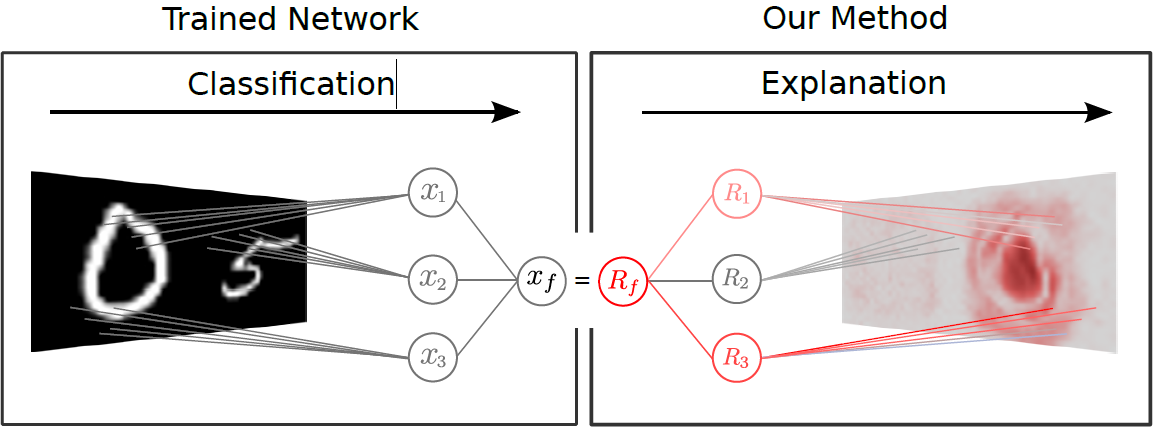
\includegraphics[height=2.5cm, width=8cm]{image/fig._1_example}

\end{figure}
\end{frame}


\begin{frame}
\frametitle{Example MNIST: Heatmaps}
\vspace{0.5cm}
\begin{figure}
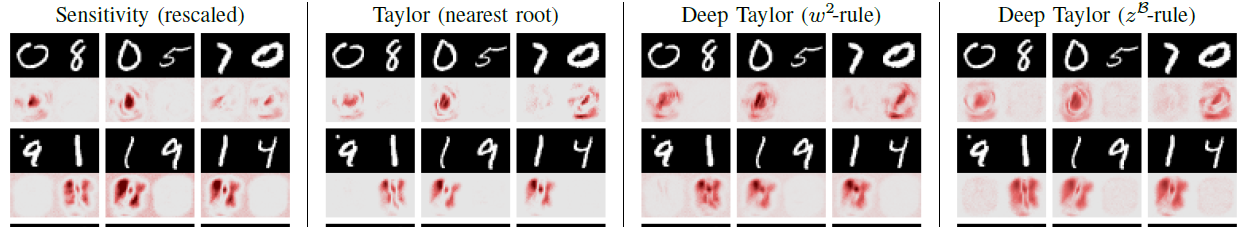
\includegraphics[height=2.5cm, width=12cm]{image/example_mnist_heatmap}
\end{figure}

\begin{figure}
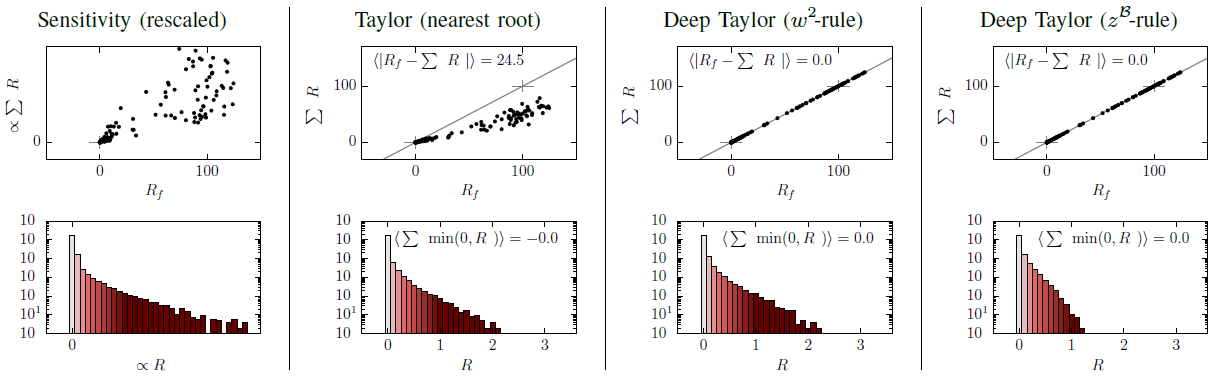
\includegraphics[height=3.25cm, width=12cm]{image/example_mnist_consistent}
\vspace{-0.75cm}
\caption{Heatmap and Empirical Results of Consistency}
\end{figure}


\end{frame}



\section[Application to Deep Networks]{Application to Deep Networks}


\begin{frame}
\frametitle{Deep Networks}
Many problems require very complex deep architectures

\begin{figure}
\label{fig1}
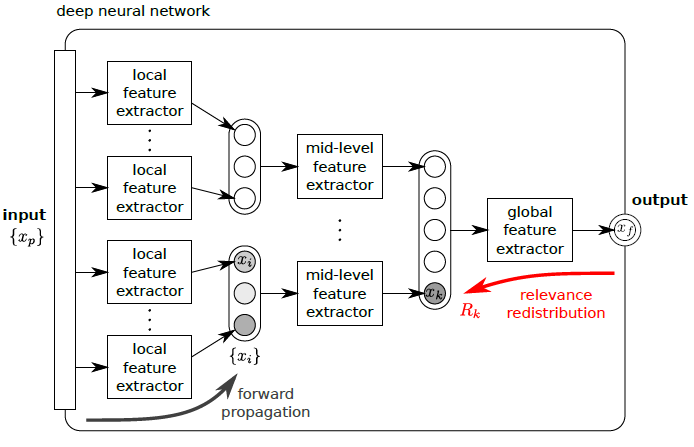
\includegraphics[height=6cm, width=11cm]{image/example_deep_network_one}
\vspace{-0.25cm}
\caption{Example Deep Network}

\end{figure}

\vspace{-1cm}
\end{frame}

\iffalse
\begin{frame}
\frametitle{Relevance Model}
\vspace{0.25cm}
In deep architectures as in figure 3 a mapping between two layers may be unknown, even if it exists
\begin{block}{Definition 1}
A relevance model is a function that maps a set of neuron activations at a given layer to the relevance of a neuron in a higher layer, and whose output can be redistributed onto its input variables.
\end{block}

\begin{figure}
\label{fig1}
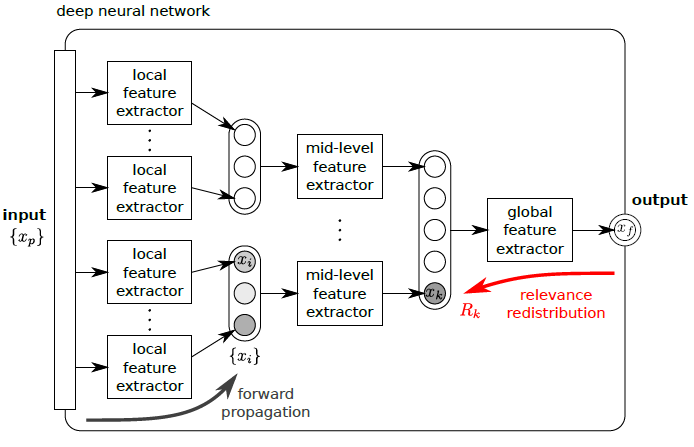
\includegraphics[height=4cm, width=7.75cm]{image/example_deep_network_one}
\end{figure}
\vspace{-0.5cm}
\end{frame}
\fi

\begin{frame}
\frametitle{Min-Max Relevance Model}
\vspace{0.4cm}
Trainable relevance model defined as
\begin{align*}
y_j &= \max(0,\sum_ix_iv_{ij} + a_j)\\
\hat{R}_k &= \sum_j y_j,
\end{align*}
where $a_j = \min(0,\sum_l R_l v_{lj} + d_j)$ is a negative bias
\vspace{-0.25cm}


 \begin{columns}
          \begin{column}{5cm}
          		$\rightarrow$ Compute $\{v_{ij}, v_{lj},d_j\}$ by minimizing 
			\begin{equation*}
			\min\langle (\hat{R}_k-R_k)^2) \rangle
			\end{equation*}
            \end{column} 
            \begin{column}{6cm}
			\begin{figure}
			\label{fig1}
			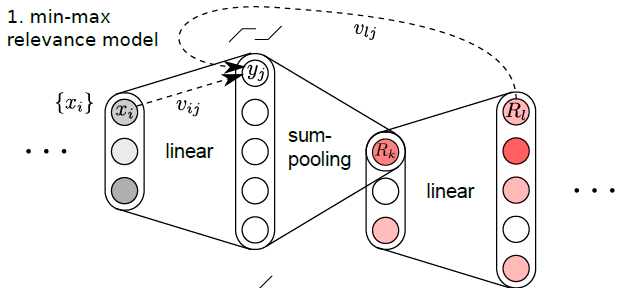
\includegraphics[height=3cm, width=6.5cm]{image/min_max_relevance_model}
			\end{figure}
	\end{column}
\end{columns} 

\end{frame}



\begin{frame}
\frametitle{Min-Max Relevance Model}
Due to the similar structure we can apply the propagation rules for the one-layer neural network
\begin{itemize}
\item Pooling layer
\begin{equation*}
R_j = y_j
\end{equation*}

\item Detection layer
\begin{equation*}
R_i = \sum_j \frac{q_{ij}}{\sum_{i'} q_{i'j}} R_j
\end{equation*}
where $q_{ij}= v_{ij}^2$, $q_{ij}= x_i v_{ij}^+$ or $q_{ij}= x_i v_{ij} - l_i v_{ij}^+ - h_i v_{ij}^-$ for the $w^2$-rule, $z^+$-rule and the $z^b$- rule respectively
\end{itemize}
\vspace{0.5cm}

$\rightarrow$ The Min-Max relevance model is due to the minimization only approximately consistent
\end{frame}



\begin{frame}
\frametitle{Training-Free Relevance Model}
Consider the original network structure
\begin{align*}
x_j &= \max(0,\sum_ix_i w_{ij} + b_j)\\
x_k &= \norm{\{x_j\}}_p
\end{align*}
If the upper layer was explained by the $z^+$-rule, relevance $R_k$ can be written as


 \begin{columns}
          \begin{column}{5cm}
			\begin{align*}
			R_k &= \sum_l \frac{x_k w_{kl}^+}{\sum_{k'} x_{k'} w_{k'l}^+} R_l\\
				&= \bigl( \sum_j x_j \bigr)\cdot \frac{\norm{\{x_j\}}_p}{\norm{\{x_j\}}_1}   \sum_l \frac{w_{kl}^+R_l}{\sum_{k'} x_{k'} w_{k'l}^+} 
			\end{align*}
            \end{column} 
            \begin{column}{5cm}
			\begin{figure}
			\label{fig1}
			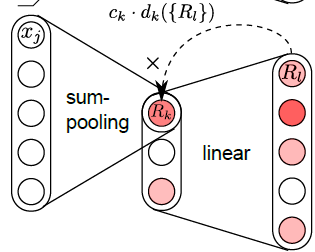
\includegraphics[height=3cm, width=4cm]{image/training-free_relevance_model_3}
			\end{figure}
	\end{column}
\end{columns} 

\end{frame}



\begin{frame}
\frametitle{Training-Free Relevance Model}
\vspace{0.25cm}
As before we can apply the propagation rules for the one-layer neural network
\begin{itemize}
\item Pooling layer
\begin{equation*}
R_j = \frac{x_j}{\sum_{j'} x_{j'}}R_k
\end{equation*}

\item Detection layer
\begin{equation*}
R_i = \sum_j \frac{q_{ij}}{\sum_{i'} q_{i'j}} R_j
\end{equation*}
where $q_{ij}= w_{ij}^2$, $q_{ij}= x_i w_{ij}^+$ or $q_{ij}= x_i w_{ij} - l_i w_{ij}^+ - h_i w_{ij}^-$ for the $w^2$-rule, $z^+$-rule and the $z^b$- rule respectively
\end{itemize}
\vspace{0.1cm}
$\rightarrow$ The training-free relevance model is consistent\\

\vspace{0.5cm}
When using the training-free model for the whole network all but the first layer need to be decomposed using the $z^+$-rule
\end{frame}


\section{Python Programming Example}

\begin{frame}
\frametitle{Relevance Distribution on the Titanic Dataset}
\vspace{0.5cm}
\begin{figure}
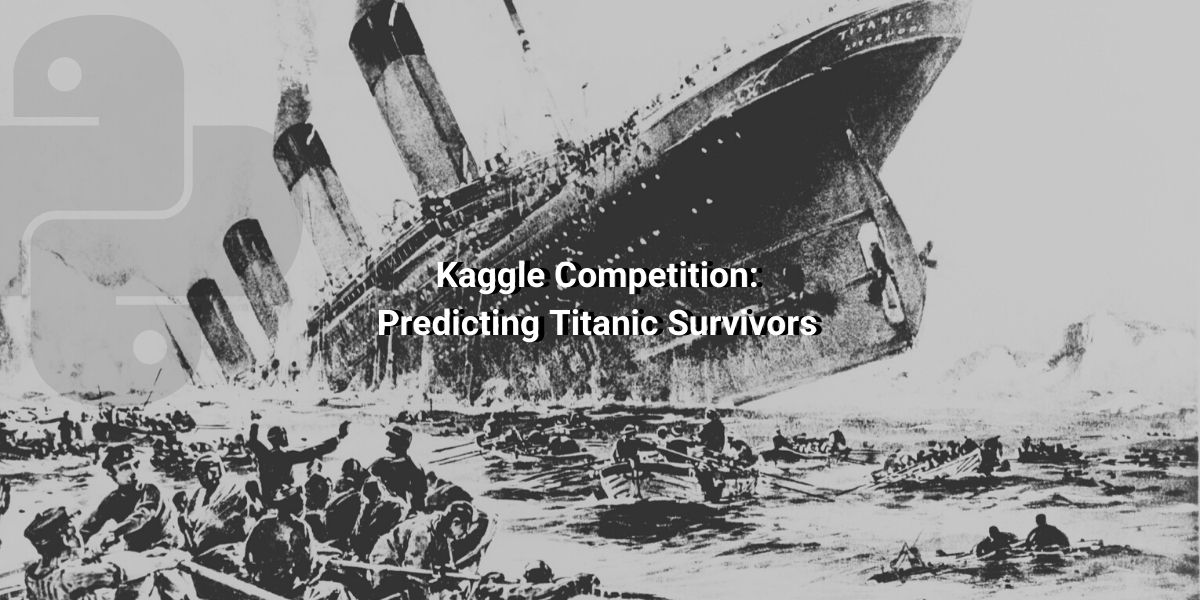
\includegraphics[height=5cm, width=11cm]{image/kaggle_titanic_challenge}
\end{figure}
\vspace{0.25cm}
\url{https://github.com/mpommer/Deep-Taylor-Decomposition-Python}
\end{frame}


\begin{frame}[allowframebreaks]
\frametitle{References}
% This prints the bibliography on the slide
\printbibliography
\end{frame}






\end{document}